\documentclass[11pt,a4paper]{article}
\usepackage[utf8]{inputenc}
\usepackage[spanish]{babel}
\usepackage{graphicx}
\usepackage{hyperref}
\usepackage{amsmath}
\usepackage{booktabs}
\usepackage[margin=2.5cm]{geometry}
\usepackage{caption}
\usepackage{float}
\usepackage{subcaption}

\captionsetup{justification=centering}

\title{\textbf{Explicabilidad y Detección de Shortcut Learning en Clasificación de Neumonía por Rayos X}}
\author{Proyecto Final - Ética y Explicabilidad de la IA \\ Francisco Javier Ríos}
\date{Diciembre 2025}

\begin{document}

\maketitle

\begin{abstract}
    Este trabajo investiga la aplicabilidad de técnicas de Inteligencia Artificial Explicable (XAI) en la detección de neumonía mediante imágenes de rayos X torácicos. Se entrena un modelo baseline basado en ResNet-18 preentrenado y se compara con un modelo intencionalmente afectado por \textit{shortcut learning}. Mediante técnicas como Grad-CAM y Activation Maximization, se demuestran diferencias en las características aprendidas por ambos, y cómo éstas no son evidentes mediante métricas tradicionales (como \textit{accuracy} en un cierto conjunto de datos). Los resultados subrayan la importancia crítica de XAI en aplicaciones médicas para garantizar que los modelos aprendan patrones clínicamente relevantes. Todos los códigos y datos están disponibles en \url{https://github.com/Javirios03/final_project_xai}.
\end{abstract}

\section{Introducción}

La aplicación de deep learning en diagnóstico médico ha mostrado resultados prometedores, pero plantea desafíos éticos y de confiabilidad \cite{rudin2019stop}. Los modelos pueden aprender correlaciones espurias (\textit{shortcut learning}) \cite{geirhos2020shortcut} en lugar de patrones clínicamente relevantes, comprometiendo su generalización y seguridad.

Este proyecto tiene tres objetivos principales: (1) desarrollar un modelo de clasificación de neumonía interpretable, (2) demostrar experimentalmente el fenómeno de shortcut learning mediante corrupción controlada de datos, y (3) validar técnicas XAI para detectar estos comportamientos no deseados.

\section{Datos y Metodología}

\subsection{Dataset}

Se utiliza el dataset Chest X-Ray Pneumonia de Kaggle \cite{kermany2018chest}, que contiene 5.856 radiografías torácicas en escala de grises con dos clases: NORMAL (27\%) y PNEUMONIA (73\%). La distribución presenta un desbalance significativo de 2.71:1 a favor de la clase PNEUMONIA.

Los datos se dividen en 85\% entrenamiento (4,434 imágenes), 15\% validación (782 imágenes) y un conjunto de test fijo (624 imágenes). Las imágenes presentan dimensiones variables (384-2916 píxeles de ancho), requiriendo redimensionamiento a 224×224 píxeles para compatibilidad con ResNet-18.

\subsection{Arquitectura del Modelo}

Se emplea ResNet-18 preentrenado en ImageNet \cite{he2016deep}, modificando la capa final para clasificación binaria. El preentrenamiento proporciona características visuales robustas que facilitan el transfer learning. Durante el entrenamiento se aplica:

\begin{itemize}
    \item Data augmentation: flip horizontal (p=0.5), rotación (±10°), jitter de brillo/contraste
    \item Optimizador: AdamW con learning rate inicial de $10^{-4}$ y decaimiento de peso (\textit{weight decay}) de $10^{-4}$
    \item Función de pérdida: CrossEntropyLoss con pesos de clase balanceados
    \item Early stopping con paciencia de 3 épocas
\end{itemize}

\subsection{Generación de Shortcut Learning}

Para estudiar el fenómeno de forma controlada, se crea un segundo modelo entrenado desde cero (sin preentrenamiento \footnote{En pruebas iniciales, se intentó hacer con preentrenamiento, pero el modelo no aprendía los atajos deseados (probablemenente debido a que ya había aprendido características robustas que impedían la dependencia de atajos espurios durante el preentrenamiento)}) sobre un dataset corrupto. Se añaden marcadores circulares blancos en la esquina superior izquierda únicamente a imágenes de la clase PNEUMONIA durante entrenamiento. Este artefacto artificial actúa como un \textit{shortcut} espurio correlacionado perfectamente con la clase objetivo.

\begin{figure}[h]
    \centering
    \includegraphics[width=0.65\textwidth]{figures/04_corruption_comparison.png}
    \caption{Ejemplos de imágenes originales vs. corruptas con marcador artificial}
    \label{fig:corruption}
\end{figure}

\subsection{Entrenamiento y Evaluación}

Ambos modelos (baseline y shortcut) se entrenan, respectivamente, durante 20 y 15 épocas hasta convergencia. De cara a diagnosticar un posible sobreajuste, se monitorean las curvas de pérdida y accuracy en entrenamiento y validación (Figura \ref{fig:overfitting_sub1}). Adicionalmente, se evalúa el rendimiento en datos limpios y corruptos para cuantificar el impacto del shortcut learning.

Como podemos observar en la Figura \ref{fig:overfitting_sub2}, el modelo baseline alcanza un accuracy del 81.57\% en datos limpios, mientras que el modelo shortcut logra un 98.88\% en datos corruptos pero sólo un 46.47\% en datos limpios, evidenciando su dependencia del marcador artificial.

\begin{figure}[H]
    \centering

    % Fila superior: dos imágenes lado a lado
    \begin{subfigure}[c]{0.48\textwidth}
        \centering
        \includegraphics[width=\textwidth]{figures/06_overfitting_check.png}
        \caption{Evolución de las funciones de pérdida y accuracy durante el entrenamiento (Baseline)}
        \label{fig:overfitting_sub1}
    \end{subfigure}
    \hfill
    \begin{subfigure}[c]{0.48\textwidth}
        \centering
        \includegraphics[width=\textwidth]{figures/07_shortcut_learning_comparison.png}
        \caption{Comparación de rendimiento entre modelo baseline y shortcut}
        \label{fig:overfitting_sub2}
    \end{subfigure}
    \caption{Análisis de sobreajuste y rendimiento entre modelos}
    \label{fig:overfitting}
\end{figure}

Algo a destacar es que, si bien el modelo baseline alcanza un accuracy que no es sobresaliente (81.57\%), sus métricas de recall (99.23\%) y AUC (0.9487) son elevadas (\ref{sec:appendix_metrics}), lo que indica que el modelo es capaz de identificar casi todos los casos positivos de neumonía, aunque a costa de una mayor tasa de falsos positivos. Esto es crucial en aplicaciones médicas donde la sensibilidad es prioritaria (el coste derivado de falsos negativos es mucho mayor que el de falsos positivos).

\section{Técnicas XAI Aplicadas}

De cara a interpretar y comparar ambos modelos, hemos seleccionado dos técnicas de XAI, una local/híbrida (Grad-CAM) y otra global (Activation Maximization):

\subsection{Grad-CAM (Gradient-weighted Class Activation Mapping)}

Grad-CAM \cite{selvaraju2017gradcam} visualiza las regiones de una imagen concreta que más contribuyen a la decisión del modelo mediante el cálculo de gradientes de la clase objetivo respecto a los mapas de activación de la última capa convolucional. De esta forma, se generan mapas de calor superpuestos a la imagen original que indican las áreas de mayor atención del modelo.

\begin{figure}[h]
    \centering
    \begin{subfigure}[b]{\textwidth}
        \centering
        \includegraphics[width=0.55\textwidth]{figures/08_gradcam_pneumonia_clean.png}
    \end{subfigure}

    \vspace{0.5cm}

    \begin{subfigure}[b]{\textwidth}
        \centering
        \includegraphics[width=0.55\textwidth]{figures/09_gradcam_pneumonia_corrupt.png}
    \end{subfigure}
    \caption{Comparación de mapas Grad-CAM para un caso de PNEUMONIA: (arriba) imagen limpia, (abajo) imagen corrupta con marcador artificial}
    \label{fig:gradcam}
\end{figure}

El modelo baseline enfoca correctamente en el área pulmonar, específicamente el lóbulo inferior derecho, donde se observan opacidades características de neumonía. Dicha atención no cambia radicalmente al introducir el marcador artificial. En contraste, en el caso de la imagen corrupta, el modelo shortcut concentra toda su atención en el marcador circular y, en la imagen limpia, no muestra atención significativa en ninguna región relevante.

\vspace{0.5cm}

En adición a este análisis cualitativo, realizamos un estudio cuantitativo de Grad-CAM sobre múltiples ejemplos, obteniendo un mapa de calor promediado a lo largo de 100 imágenes de la clase PNEUMONIA:

\begin{figure}[h]
    \centering
    \includegraphics[width=0.6\textwidth]{figures/12_average_gradcam_comparison.png}
    \caption{Mapa de calor promedio de Grad-CAM sobre 100 imágenes de PNEUMONIA}
    \label{fig:avg_gradcam}
\end{figure}

El modelo baseline muestra atención distribuida por todo el campo pulmonar, sin focos de activación extrema, lo cual es consistente con la variabilidad clínica de la neumonía. Sin embargo, el modelo shortcut presenta un comportamiento totalmente diferente. Es interesante analizar cómo cambia la atención al comparar imágenes limpias y corruptas: en imágenes limpias, parece centrarse en el cuadrante inferior derecho (lo cual parece indicar que, si bien el grueso de lo aprendido es el marcador, el modelo también intenta buscar alguna característica médica en ausencia del atajo). En imágenes corruptas, la atención se concentra exclusivamente en la esquina superior izquierda, donde se encuentra el marcador artificial, ignorando completamente el resto de la imagen.

Este análisis refuerza la conclusión de que el modelo shortcut no aprende características médicas relevantes (que el baseline sí capta), eliminando ruido de casos específicos. Sin embargo, debemos tener en cuenta las limitaciones inherentes a Grad-CAM: aunque es intuitivo para humanos, no garantiza una fidelidad absoluta al proceso de decisión del modelo \cite{adebayo2018sanity}. Adicionalmente, obtener el mapa de calor promedio puede diluir detalles importantes sobre la heterogeneidad de casos individuales. Esto implica que no podemos distinguir, a falta de un análisis más profundo, si nuestros modelos miran consistentemente regiones relevantes o si alterna aleatoriamente entre distintas áreas o estrategias.

\subsection{Activation Maximization}

Si bien Grad-CAM ofrece una visión local del comportamiento del modelo, necesitamos responder a la pregunta: ¿qué características globales ha aprendido el modelo para representar cada clase? Para ello, utilizamos Activation Maximization \cite{actmax2009,zhu2025representationunderstandingactivationmaximization}, una técnica que sintetiza imágenes que maximizan la activación de una clase específica en el modelo, produciendo un prototiopo visual de lo que el modelo asocia con dicha clase.

\begin{figure}[htbp]
    \centering
    % Primera fila
    \begin{subfigure}[b]{0.48\textwidth}
        \centering
        \includegraphics[width=\textwidth]{figures/15_am_baseline_normal.png}
        \caption{Baseline - Clase NORMAL}
        \label{fig:am_baseline_normal}
    \end{subfigure}
    \hfill
    \begin{subfigure}[b]{0.48\textwidth}
        \centering
        \includegraphics[width=\textwidth]{figures/16_am_baseline_pneumonia.png}
        \caption{Baseline - Clase PNEUMONIA}
        \label{fig:am_baseline_pneumonia}
    \end{subfigure}

    \vspace{1em} % Espacio vertical entre filas

    % Segunda fila
    \begin{subfigure}[b]{0.48\textwidth}
        \centering
        \includegraphics[width=\textwidth]{figures/17_am_shortcut_normal.png}
        \caption{Shortcut - Clase NORMAL}
        \label{fig:am_shortcut_normal}
    \end{subfigure}
    \hfill
    \begin{subfigure}[b]{0.48\textwidth}
        \centering
        \includegraphics[width=\textwidth]{figures/18_am_shortcut_pneumonia.png}
        \caption{Shortcut - Clase PNEUMONIA}
        \label{fig:am_shortcut_pneumonia}
    \end{subfigure}

    \caption{Imágenes sintetizadas mediante Activation Maximization para ambas clases y modelos}
    \label{fig:activation_maximization}
\end{figure}

En la figura superior, observamos 4 imágenes sintetizadas por clase y modelo. Analizándolas por separado:
\begin{itemize}
    \item \textbf{Modelo Baseline}:
          \begin{itemize}
              \item \textit{Clase NORMAL}: Las imágenes sintetizadas muestran estructuras que recuerdan costillas (líneas blancas horizontales y verticales) con una cierta simetría bilateral y apariencia anatómica (se parecen, si bien vagamente, a una radiografía torácica normal). Esto parece indicar que el modelo ha aprendido que la presencia de estas estructuras es indicativa de una radiografía normal (en la cual no existen opacidades ni anomalías visibles que oculten dichas estructuras).
              \item \textit{Clase PNEUMONIA}: Cabe destacar que dichas imágenes son relativamente uniformes y una intensidad media-baja. Esto sugiere que el modelo se guía por texturas complejas de bajo nivel que no son fácilmente interpretables por el ojo humano, lo cual conecta con una de las mayores limitaciones al tratar de explicar modelos de visión por ordenador: esa diferencia tan marcada entre \textit{faithfulness} y \textit{plausibility} que estudiamos a lo largo del curso. Intentar simplificar el razonamiento del modelo a mecanismos antropocéntricos (formas reconocibles, objetos familiares) puede ser engañoso, ya que el modelo puede estar utilizando patrones estadísticos complejos que no son evidentes para humanos.
          \end{itemize}
    \item \textbf{Modelo Shortcut}:
          Respecto al modelo shortcut, los prototipos generados para ambas clases son muy similares entre sí y presentan patrones que más bien parecen ruido aleatorio, sin estructuras reconocibles ni características anatómicas claras. Esto refuerza la conclusión de que el modelo no ha aprendido características médicas relevantes, sino que se basa en el marcador artificial.
\end{itemize}

Adicionalmente, es importante mencionar los \textit{scores} obtenidos durante la optimización de Activation Maximization (ver Apéndice \ref{sec:appendix_am_scores}). El modelo baseline alcanza scores significativamente más altos (40 para PNEUMONIA y 13 para NORMAL) en comparación con el modelo shortcut (2.5 para NORMAL y -2.5 para PNEUMONIA). Esto indica que el modelo baseline tiene una representación más robusta y diferenciada de las clases, mientras que el modelo shortcut no logra generar activaciones fuertes, reflejando su dependencia en un atajo espurio.

No sólo eso, sino que el hecho de que el score para la clase PNEUMONIA en el modelo shortcut sea negativo (-2.5) sugiere que el modelo tiene una dificultad extrema para generar imágenes de esa clase sin la presencia del marcador artificial. Analizando esto más en detalle, dado que el método de Activation Maximization aplica regularizaciones y desenfoques periódicamente, dicha optimización no es capaz de encontrar una solución tan específica que requiere:
\begin{enumerate}
    \item La presencia del marcador artificial (un círculo perfecto)
    \item Con una intensidad muy concreta (blanco puro)
    \item En una localización concreta (esquina superior izquierda)
\end{enumerate}

\section{Sanity Checks y Actionable Insights}

\subsection{Validación mediante Sanity Checks}

De cara a validar la fidelidad de las explicaciones obtenidas mediante Grad-CAM, hemos implementado un \textit{sanity check} basado en la metodología propuesta por Adebayo et al. \cite{adebayo2018sanity}, consistente en randomizar los pesos del modelo \footnote{En este caso, nos limitamos a aplicarlo al modelo baseline, ya que el modelo shortcut no presenta mapas de atención coherentes desde el inicio} y observar cómo cambian las visualizaciones de Grad-CAM:

\begin{figure}[h]
    \centering
    \includegraphics[width=0.6\textwidth]{figures/14_sanity_check_randomization.png}
    \caption{Sanity check de Grad-CAM mediante randomización de pesos}
    \label{fig:sanity_check}
\end{figure}

De este análisis, concluimos que las visualizaciones de Grad-CAM son efectivamente sensibles a los pesos del modelo. La confianza del modelo en su predicción colapsa a un 50,2\% (en esencia, un clasificador aleatorio en este problema binario) tras la randomización, y las regiones de atención se vuelven muy débiles. Todo ello indica que las explicaciones obtenidas reflejan fielmente el razonamiento aprendido por el modelo, reforzando la validez de los análisis previos.

\subsection{Aplicaciones prácticas para Aplicaciones Médicas}

Los resultados detallados en las anteriores secciones subrayan la importancia crítica de incorporar técnicas XAI en el desarrollo y despliegue de modelos de IA en contextos médicos. Basándonos en estos hallazgos, proponemos las siguientes recomendaciones prácticas:

\begin{enumerate}
    \item \textbf{Validación obligatoria con XAI}: El uso de técnicas como Grad-CAM y Activation Maximization deja de ser un extra útil para convertirse en un requisito indispensable en la validación de modelos médicos
    \item \textbf{Inspección de datos}: Los datasets médicos deben auditarse para detectar correlaciones espurias (marcadores institucionales, artefactos de adquisición, sesgos demográficos)
    \item \textbf{Transfer learning con precaución}: El preentrenamiento en ImageNet aporta robustez contra shortcuts, pero no elimina completamente el riesgo
    \item \textbf{Evaluación en distribuciones múltiples}: Los modelos deben validarse en datos de diferentes instituciones y equipos radiológicos
\end{enumerate}
\newpage
\section{Limitaciones y Discusión}

\subsection{Limitaciones del Estudio}

Si bien los resultados obtenidos derivan en conclusiones valiosas, es importante reconocer las limitaciones inherentes a nuestro proyecto:

\subsubsection{Interpretación humana frente a fidelidad del modelo}

Las visualizaciones de Grad-CAM y las imágenes sintetizadas mediante Activation Maximization, si bien visualmente intuitivas, presentan una limitación inherente: el privilegio de la plausibilidad frente a la fidelidad al razonamiento interno. Los mapas de atención muestran regiones de alta activación en \textit{feature maps} de capas convolucionales, pero dicha activación es una correlación, no necesariamente una prueba causal del proceso de decisión del modelo.

Como se discute en \cite{adebayo2018sanity}, el uso indiscriminado de explicaciones visuales puede inducir a conclusiones erróneas, especialmente si los usuarios finales (médicos, reguladores) no están plenamente conscientes de las limitaciones de estas técnicas. Adicionalmente, existen algunas restricciones metodológicas relacionadas con las técnicas empleadas. Por ejemplo, el uso de la activación ReLU en Grad-CAM elimina activaciones negativas, lo cual puede ocultar regiones que el modelo podría usar como evidencia en contra de una clase.

Respecto a Activation Maximization, la optimización de imágenes sintetizadas depende fuertemente de las regularizaciones aplicadas (desenfoque, penalizaciones de norma). Asimismo, dichos prototipos muestran texturas de bajo nivel que no son fácilmente interpretables por humanos, lo cual limita su utilidad práctica en entornos clínicos (mostrando la otra cara de la moneda del trade-off entre plausibility y faithfulness).

\subsubsection{Simplificación experimental}

El uso de un marcador artificial para inducir shortcut learning, si bien efectivo para demostrar el fenómeno, es una simplificación que puede no capturar la complejidad de shortcuts reales en datos médicos. En escenarios clínicos, dichos shortcuts suelen no ser tan obvios y pueden involucrar múltiples factores sutiles (diferencias en protocolos de adquisición, demografía del paciente, artefactos específicos de equipos). Esta simplificación facilita la demostración del fenómeno, pero puede limitar la generalización de los hallazgos a situaciones del mundo real.

\subsubsection{Tamaño y diversidad del dataset}

Por otro lado, el dataset utilizado, aunque adecuado para propósitos experimentales, presenta limitaciones en cuanto a tamaño y diversidad. Un total de 5.856 imágenes puede no ser representativo de la variabilidad clínica completa de la neumonía, y la distribución desbalanceada de clases podría influir en el aprendizaje del modelo (en este caso, induciendo un sesgo intrínseco hacia la clase mayoritaria, PNEUMONIA). Estudios futuros deberían considerar datasets más grandes y diversos para validar la robustez de las conclusiones.

\subsubsection{Ausencia de Validación Clínica}

Finalmente, es crucial destacar que este estudio carece de validación clínica directa. Si bien las técnicas XAI proporcionan insights valiosos sobre el comportamiento del modelo, la interpretación y utilidad de estas explicaciones debe ir acompañada de la experiencia de profesionales médicos (a la cual debemos remitir, en última instancia, para justificar la relevancia de nuestros hallazgos). Por lo tanto, es nuestra opinión que toda conclusión obtenida mediante modelos de IA debe ser supeditada a la revisión y validación por parte de expertos clínicos.

\subsection{Implicaciones Éticas}

El fenómeno estudiado a lo largo de este proyecto tiene profundas implicaciones éticas en el contexto de la IA médica. La dependencia de shortcuts espurios puede conducir a consecuencias potencialmente desastrosas:

\begin{itemize}
    \item Fallar catastróficamente al ser desplegado en instituciones con diferentes equipos/protocolos
    \item Generar falsa confianza en profesionales médicos al mostrar alta precisión en validación
    \item Comprometer la seguridad del paciente al basar decisiones en correlaciones no clínicas
\end{itemize}

De igual modo, la ciega confianza en explicaciones XAI sin una comprensión crítica de sus limitaciones puede inducir a errores de interpretación. La falta de esto último puede radicar en una falsa sensación de seguridad, llevando a decisiones clínicas erróneas basadas en explicaciones engañosas.

\section{Conclusiones}

Nuestro proyecto demuestra experimentalmente la efectividad de técnicas XAI para detectar shortcut learning en clasificación de imágenes médicas. Sintetizamos algunos hallazgos clave:

\begin{enumerate}
    \item El modelo baseline basado en transfer learning aprende características anatómicas relevantes, evidenciado por Grad-CAM que enfoca en regiones pulmonares y Activation Maximization que genera prototipos con estructuras reconocibles

    \item El modelo shortcut, entrenado desde cero con datos corruptos, depende exclusivamente del marcador artificial, alcanzando 98.9\% de precisión en datos corruptos pero solo 46.5\% en datos limpios

    \item Los sanity checks validan que las explicaciones XAI reflejan fielmente el razonamiento aprendido por los modelos

    \item El preentrenamiento en ImageNet proporciona robustez contra shortcuts simples, aunque no es una solución universal
\end{enumerate}

En conclusión, XAI no es opcional en aplicaciones médicas de IA: es una necesidad técnica y ética para garantizar que los modelos aprendan patrones clínicamente relevantes en lugar de correlaciones espurias. La combinación de múltiples técnicas de explicabilidad (Grad-CAM, Activation Maximization, sanity checks) proporciona una visión más completa y confiable del comportamiento del modelo.

\newpage

\appendix

\section{Ilustraciones Adicionales}
\label{sec:appendix_figures}

Si bien no incluimos todas las figuras en el cuerpo principal del informe (en pos de la brevedad), proponemos una serie de ilustraciones complementarias que pueden facilitar la comprensión de los conceptos tratados:

\subsection{Visualización del Dataset}
\label{sec:appendix_dataset}

\begin{figure}[htbp]
    \centering

    % Fila superior: dos imágenes lado a lado
    \begin{subfigure}[b]{0.48\textwidth}
        \centering
        \includegraphics[width=\textwidth]{figures/01_class_distribution.png}
        \caption{Distribución de clases en el dataset}
        \label{fig:sub1}
    \end{subfigure}
    \hfill
    \begin{subfigure}[b]{0.48\textwidth}
        \centering
        \includegraphics[width=\textwidth]{figures/02_image_properties.png}
        \caption{Propiedades de las imágenes (tamaños y formatos)}
        \label{fig:sub2}
    \end{subfigure}

    % Salto de línea
    \vspace{0.5cm}

    % Fila inferior: una imagen más ancha
    \begin{subfigure}[b]{0.9\textwidth}
        \centering
        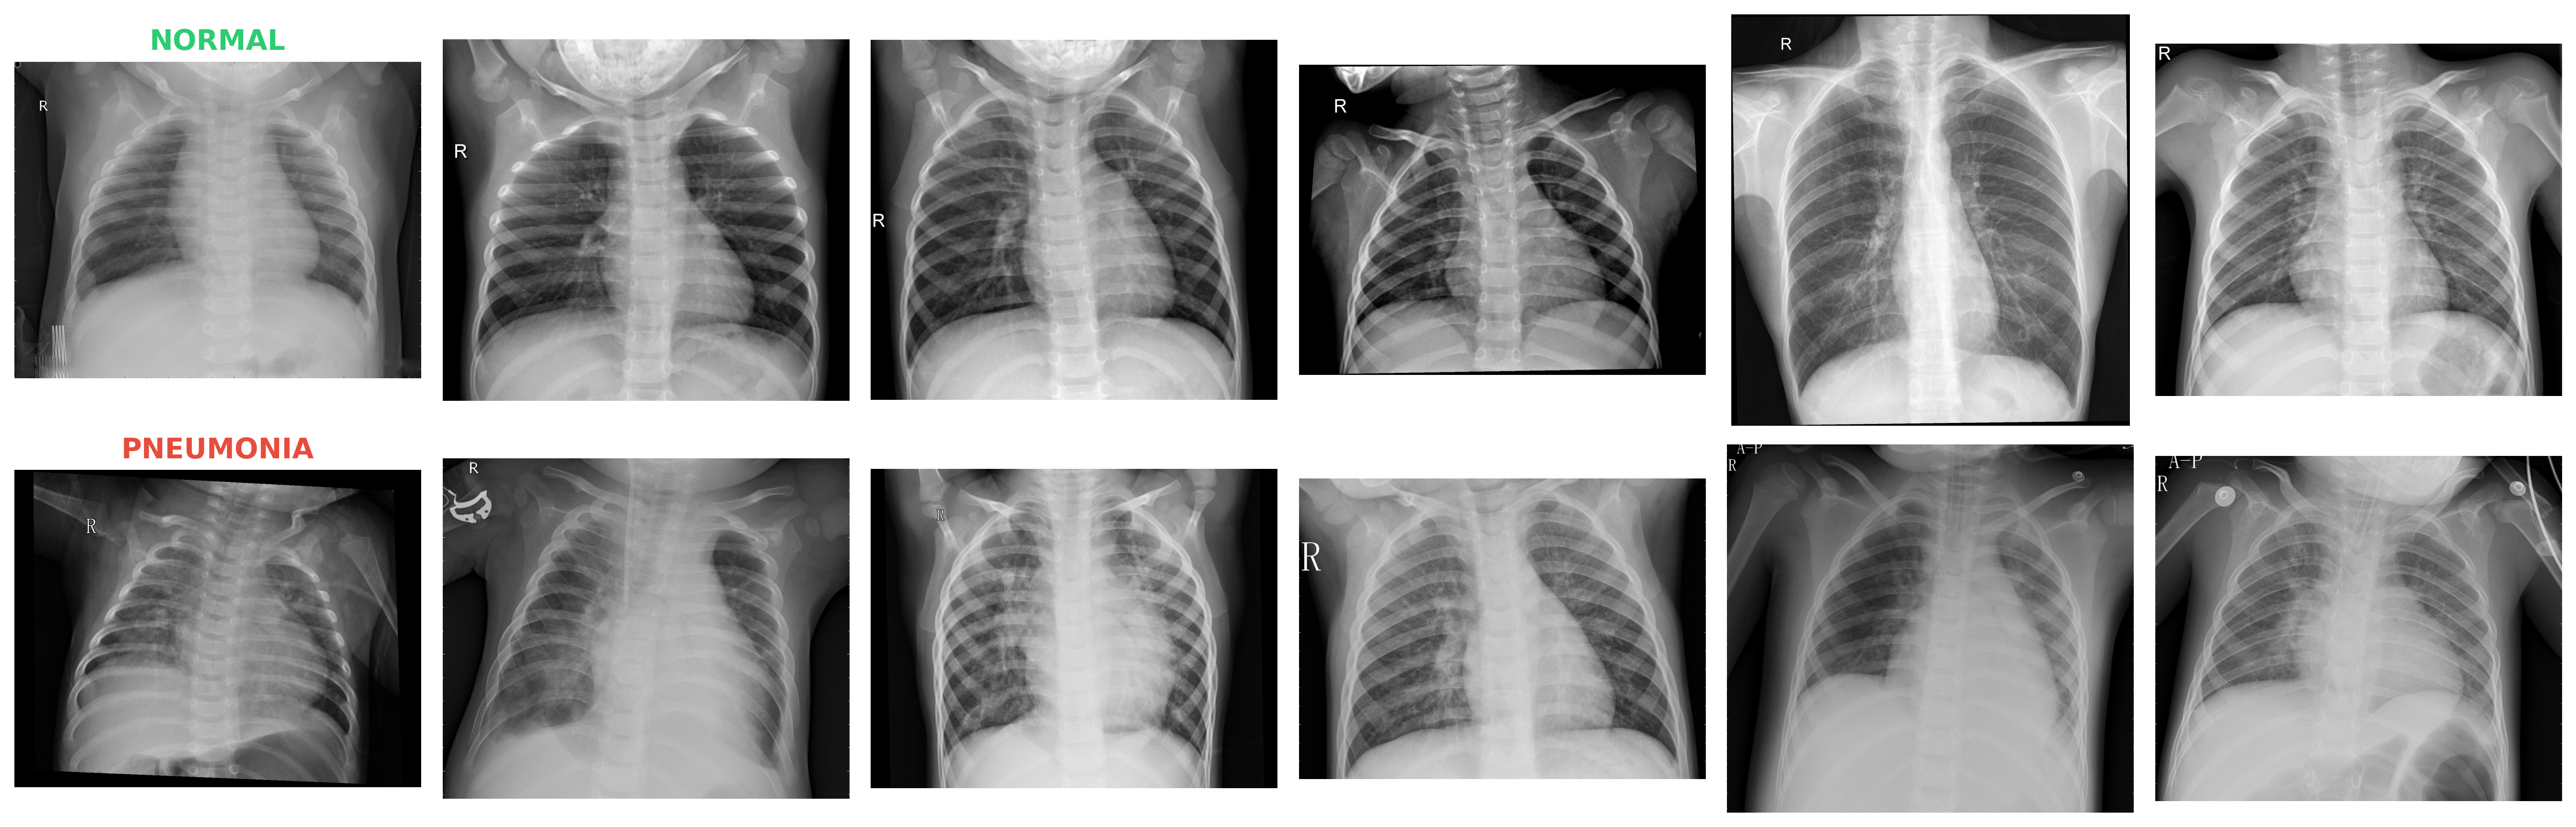
\includegraphics[width=\textwidth]{figures/03_sample_images.png}
        \caption{Imágenes de muestra del dataset}
        \label{fig:sub3}
    \end{subfigure}

    \caption{Información visual adicional sobre el dataset utilizado}
    \label{fig:tres_imagenes}
\end{figure}
\newpage
\subsection{Visualizaciones de Grad-CAM Complementarias}
\label{sec:appendix_gradcam}

\begin{figure}[htbp]
    \centering
    \begin{subfigure}[b]{0.48\textwidth}
        \centering
        \includegraphics[width=\textwidth]{figures/10_gradcam_multiple_examples_clean.png}
    \end{subfigure}
    \hfill
    \begin{subfigure}[b]{0.48\textwidth}
        \centering
        \includegraphics[width=\textwidth]{figures/11_gradcam_multiple_pneumonia_corrupt.png}
    \end{subfigure}
    \caption{Visualizaciones de Grad-CAM complementarias en casos de neumonía: (izquierda) imágenes limpias, (derecha) imágenes corruptas}
    \label{fig:gradcam_complementarias}
\end{figure}

\subsection{Distribución de la atención Grad-CAM según regiones pulmonares}
\label{sec:appendix_attention_distribution}

\begin{figure}[H]
    \centering
    \includegraphics[width=0.6\textwidth]{figures/13_attention_distribution_barplot.png}
    \caption{Distribución cuantitativa de la atención Grad-CAM en diferentes regiones pulmonares}
    \label{fig:attention_distribution}
\end{figure}

\section{Métricas Detalladas de Rendimiento}

\subsection{Métricas del Modelo Baseline}
\label{sec:appendix_metrics}

\begin{table}[H]  % {l} = izquierda, ancho = 35% del texto
    \centering
    \begin{tabular}{||l|c||}
        \toprule
        \textbf{Métrica} & \textbf{Valor} \\
        \midrule
        Accuracy         & 81.57\%        \\
        Precision        & 77.56\%        \\
        Recall           & 99.23\%        \\
        F1-Score         & 87.06\%        \\
        AUC              & 0.9487         \\
        \bottomrule
    \end{tabular}
    \caption{Métricas detalladas del modelo baseline en el conjunto de test limpio}
    \label{tab:metrics}
\end{table}

\subsection{Matriz de Confusión}
\label{app:confusion_matrix}

\begin{table}[H]
    \centering
    \begin{tabular}{lcc}
        \toprule
                                 & \textbf{Pred: NORMAL} & \textbf{Pred: PNEUMONIA} \\
        \midrule
        \textbf{True: NORMAL}    & 186 (79.5\%)          & 48 (20.5\%)              \\
        \textbf{True: PNEUMONIA} & 3 (0.8\%)             & 387 (99.2\%)             \\
        \bottomrule
    \end{tabular}
    \caption{Matriz de confusión del modelo baseline en test set}
    \label{tab:confusion_matrix}
\end{table}

\section{Scores de Activation Maximization}
\label{sec:appendix_am_scores}

Los scores obtenidos (medidos en logits) para las imágenes sintetizadas mediante Activation Maximization son los siguientes:

\begin{table}[H]
    \centering
    \begin{tabular}{lcc}
        \toprule
        \textbf{Modelo} & \textbf{Clase} & \textbf{Score} \\
        \midrule
        Baseline        & NORMAL         & 13             \\
        Baseline        & PNEUMONIA      & 40             \\
        Shortcut        & NORMAL         & 2.5            \\
        Shortcut        & PNEUMONIA      & -2.5           \\
        \bottomrule
    \end{tabular}
    \caption{Scores de Activation Maximization para cada modelo y clase}
    \label{tab:am_scores}
\end{table}

\newpage

\bibliographystyle{unsrt}
\bibliography{citations}

\end{document}
